\documentclass{article}
\usepackage{natbib,graphicx,lineno}
\title{Hypothesis testing in geology}
\author{Pieter Vermeesch\footnote{School of Earth Sciences,
Birkbeck, University of London}}
\date{}
\pagestyle{empty}
\begin{document}
\linenumbers
\maketitle

Statistical tests such as Chi-square, t, and Kolmogorov-Smirnov are
useless for assessing geological hypotheses. Because the latter are
never exactly true, they always fail statistical hypothesis tests,
provided a large enough sample size is used. This point is illustrated
with a geophysical example, in which Pearson's Chi-square test implies
that earthquakes are unevenly distributed throughout the week, with
seismic activity being particularly high on Sunday.
\\

According to Karl Popper's epistemology of critical rationalism,
scientists should formulate falsifiable hypotheses rather than
producing ad hoc answers to empirical observations. In other words, we
should predict and test rather than merely explain \citep{popper1959}.
This is not always easy in historical sciences such as geology and
evolutionary biology. In fact, many geologists use exactly the
opposite approach, going on the field `with an open mind' and using
inductive methods to draw conclusions \citep{sengor2001}. Although it
is definitely a good thing to have an open mind, inductive reasoning
rarely leads to robust models. Fortunately, many Earth scientists
follow a more deductive line of reasoning. Often, statistical tests
such as Chi-square, t, or Kolmogorov-Smirnov are used to make
deductions statistically more `objective'. Such tests have been used
in a wide range of geological sub-disciplines, including geochemistry
\citep{reimann2000}, geophysics \citep{Anderson1999}, hydrology
\citep{lorup1998}, and geochronology \citep{sircombe2004}.
\\

The urge to use statistical tests stems from the apparent equivalence
of the Popperian paradigm to the so-called Neyman-Pearson paradigm of
statistics, according to which theories can be tested by formulating a
null hypothesis (H$_0$) and an alternative hypothesis (H$_a$).  Given
a quantitative data set D, the decision whether or not to reject H$_0$
in favor of H$_a$ is made on the basis of S(D), the so-called
`statistic'.  If S(D) is `unlikely' to occur under H$_0$, then H$_0$
is rejected. Examples of geological null hypotheses are: ``geochemical
distributions are (log)normally distributed'', ``Coulomb stress
changes of small earthquakes are unaffected by major seismic events'',
``the annual runoff of a catchment has remained constant'', or ``two
sand samples (A and B, say) share the same provenance''.
\\

While there are a number of practical and philosophical issues with
statistical testing and the concept of p-values \citep{ziliak2008}, I
would like to draw attention to a trivial albeit often overlooked
fact: geological null hypotheses are never true. In the provenance
example, for instance, it suffices that a single sand grain in sample
A is derived from some place not contributing to sample B for the null
hypothesis to be false. One problem with the Neyman-Pearson paradigm
as propagated by R. A. Fisher and others is the fundamental asymmetry
between H$_0$ and H$_a$: a `good' null hypothesis should be easy to
reject \citep{rice1995}. This is consistent with Popper's notion that
a good scientific theory should be provocative, easy to test and,
therefore, easy to reject. Only when a simple and elegant hypothesis
survives an onslaught of experimental tests can one be somewhat
confident of having found the `truth'. The problem with enforcing this
principle in a mathematical way is that few if any geological
hypotheses survive such tests.
\\

To illustrate this point, consider the following, seemingly plausible
null hypothesis: ``the occurrence of earthquakes does not depend on
the day of the week''. To test this hypothesis, a database of 118,415
earthquakes of magnitude 4 or greater and occurring between Friday,
January 1, 1999 and Thursday, January 1, 2009, was compiled from the
USGS website ({\tt http://earth\-quake.usgs.gov}).  The earthquakes
were tallied by weekday, resulting in a seven bin histogram (Figure
\ref{fig:1}) with bin counts varying between 16,348 (Friday) and
17,753 (Sunday), and an average of 16,916. Our null hypothesis is
mathematically equivalent to saying that this histogram is uniformly
distributed. A Chi-square test was used to evaluate the statistical
significance of the observed scatter and the departure from
uniformity. Given a set of expected and observed events (E$_i$ and
O$_i$, respectively, for 1 $\leq$ i $\leq$ 7), Pearson's Chi-square
statistic is given by X$^2$ = $\sum_i$(O$_i$-E$_i$)$^2$/E$_i$, which
is approximately $\chi^2$-distributed with 6 degrees of freedom. For
the earthquake database, X$^2$ = 94, and the corresponding p-value,
which is the likelihood of observing a result at least as extreme as
94, is less than 10$^{-16}$. Therefore, the null hypothesis has been
clearly rejected.
\\

Why did the earthquake data fail the test for uniformity? Because the
$\chi^2$-approximation gets progressively better with increasing
sample size, Pearson's Chi-square test should work particularly well
on our very large database. And this is exactly the problem: the test
is too sensitive. The outcome of statistical tests is determined by
two factors - effect size and sample size - which are lumped together
by Fisherian hypothesis tests.  Given a large enough dataset,
statistical tests such as Chi-Square will pick up any departure from
the null hypothesis, no matter how small. The non-uniformity of the
earthquake distribution could have a number of causes.  Perhaps
background noise is lower on weekends, leading to an increased
sensitivity of the seismometers? Or the tolling of church bells on
Sunday triggers false positives?  Whatever the reason is, it is
unlikely to be a geological one.  Clearly, `statistically significant'
is not the same as `geologically significant'.

\bibliography{d:/papers/biblio} \bibliographystyle{plainnat}

\clearpage

\begin{figure}[h]
  \centering
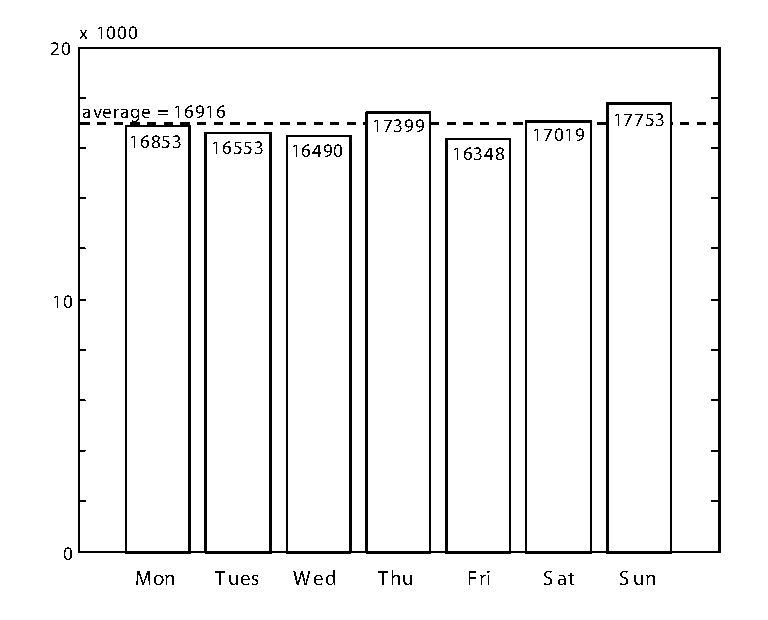
\includegraphics[width=\textwidth]{histogram-1999-2009.pdf}  
  \caption{Histogram of 118,415 earthquakes occurring between 1999
    and 2009, grouped by weekday.}
  \label{fig:1}
\end{figure}

\end{document}
